\documentclass[tikz,border=12pt]{standalone}
\usepackage[T1]{fontenc}
\usepackage[utf8]{inputenc}
\usepackage{lmodern}
\usetikzlibrary{calc}

% Tetraedro FSPC — arquivo independente, compilável com pdflatex.
% No pôster, exporte este documento como PDF ou PNG e substitua DiagramaFSPC.png.
\definecolor{ink}{HTML}{243247}
\definecolor{muted}{HTML}{64748B}
\definecolor{fun}{HTML}{7654A3}
\definecolor{str}{HTML}{C17A35}
\definecolor{pro}{HTML}{168A87}
\definecolor{con}{HTML}{3B6FAB}
\definecolor{facefront}{HTML}{DDEFE5}
\definecolor{faceside}{HTML}{C9E4DF}
\definecolor{volume}{HTML}{26734F}

\tikzset{
  edge/.style={draw=ink, line width=1.15pt, line cap=round},
  % Linha mais escura/grossa e desenhada por cima (veja abaixo), para não
  % ficar "lavada" pelo preenchimento semitransparente das faces.
  hidden edge/.style={draw=muted!85!black, line width=1.05pt, dash pattern=on 3pt off 2.2pt},
  vertex/.style={circle, draw=white, line width=1.4pt, minimum size=8pt, inner sep=0pt},
  % Estilo "cartão de vértice": caixa arredondada, borda/fundo na cor do
  % argumento, texto CENTRALIZADO (título em negrito + subtítulo em itálico),
  % no mesmo estilo usado no tetraedro FSPC anterior.
  label box/.style={
    rectangle, rounded corners=3pt, draw=#1!70!black, fill=#1!10,
    line width=0.9pt, align=center,
    text width=3.4cm, inner sep=6pt,
    font=\small
  },
  label box/.default=ink
}

\begin{document}
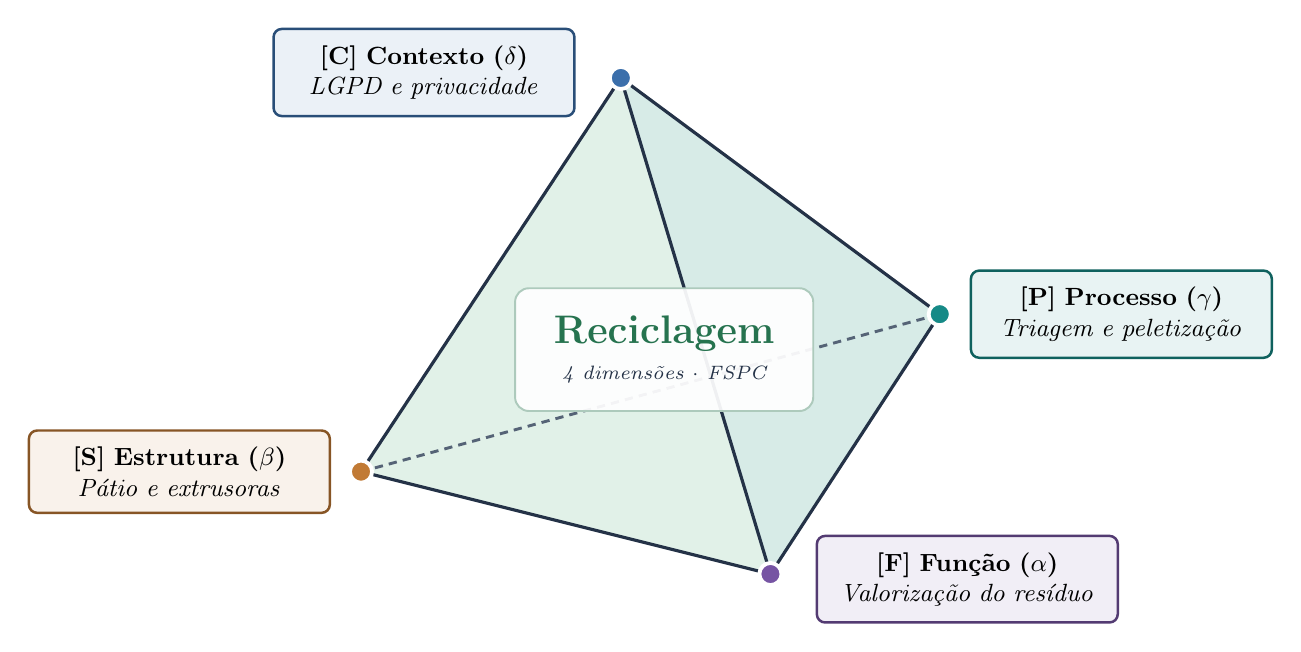
\begin{tikzpicture}[font=\sffamily]

  % Projeção: duas faces aparentes e a aresta S--P oculta.
  \coordinate (C) at (0.0,4.65);
  \coordinate (S) at (-3.30,-0.35);
  \coordinate (F) at (1.90,-1.65);
  \coordinate (P) at (4.05,1.65);

  % Cabeçalho.
%   \node[font=\bfseries\Large, text=ink] at (0.4,7.25)
%     {Tetraedro FSPC};
%   \node[font=\small, text=muted] at (0.4,6.78)
%     {Função \(\cdot\) Estrutura \(\cdot\) Processo \(\cdot\) Contexto};

  % Faces translúcidas sugerem o volume (desenhadas primeiro, no fundo).
  \fill[faceside, opacity=0.75] (C) -- (F) -- (P) -- cycle;
  \fill[facefront, opacity=0.88] (C) -- (S) -- (F) -- cycle;

  % Contorno e divisão das faces aparentes.
  \draw[edge] (C) -- (S) -- (F) -- (P) -- cycle;
  \draw[edge] (C) -- (F);

  % Aresta oculta S--P desenhada por último (por cima de tudo), para manter
  % cor/opacidade cheias em vez de ficar sob as faces translúcidas.
  \draw[hidden edge] (S) -- (P);

  % O resultado integrado fica dentro do sólido, sem confundir face e volume.
  \node[
    rounded corners=5pt, fill=white, fill opacity=0.93,
    text opacity=1, draw=volume!38, line width=0.7pt,
    inner xsep=14pt, inner ysep=10pt, align=center
  ] at (0.55,1.2) {%
    % {\scriptsize\bfseries\color{muted} VOLUME INTEGRADO}\\[3pt]
    % Serifada (igual às caixas dos vértices), com versalete + negrito
    % como "destaque" em vez de trocar de fonte.
    {\rmfamily\bfseries\Large\color{volume} Reciclagem}\\[1pt]
    {\rmfamily\itshape\color{ink}\scriptsize 4 dimensões \(\cdot\) FSPC}%
  };

  % Vértices, com cor e letra redundantes para leitura em escala de cinza.
  % Desenhados depois da aresta oculta para ficarem por cima dela também.
  \node[vertex, fill=con] at (C) {};
  \node[vertex, fill=str] at (S) {};
  \node[vertex, fill=fun] at (F) {};
  \node[vertex, fill=pro] at (P) {};

  % Cartões externos — estilo "vlabel": título em negrito + subtítulo em
  % itálico, texto centralizado, cor do vértice correspondente.
  \node[label box=con, anchor=south] at ($(C)+(-2.5,-.5)$)
    {\textbf{[C] Contexto ($\delta$)}\\ \textit{LGPD e privacidade}};

  \node[label box=str, anchor=east] at ($(S)+(-0.38,0)$)
    {\textbf{[S] Estrutura ($\beta$)}\\ \textit{Pátio e extrusoras}};

  \node[label box=fun, anchor=north] at ($(F)+(2.5,.5)$)
    {\textbf{[F] Função ($\alpha$)}\\ \textit{Valorização do resíduo}};

  \node[label box=pro, anchor=west] at ($(P)+(0.38,0)$)
    {\textbf{[P] Processo ($\gamma$)}\\ \textit{Triagem e peletização}};

%   \node[font=\scriptsize, text=muted, anchor=west]
%     at (-3.35,-3.55) {Abordagem sistêmica adaptada de Gharajedaghi (2011)};

\end{tikzpicture}
\end{document}